%9_Gauss_distribution
%notes for the course Probability and Statistics COMS10011
%taught at the University of Bristol
%2018_19 Conor Houghton conor.houghton@bristol.ac.uk
%To the extent possible under law, the author has dedicated all copyright
%and related and neighboring rights to these notes to the public domain 
%worldwide. These notes are distributed without any warranty. 

\documentclass[11pt,a4paper]{scrartcl}
\typearea{12}
\usepackage{graphicx}
%\usepackage{pstricks}
\usepackage{listings}
\usepackage{color}

\lstset{language=C}
\usepackage{fancyhdr}
\pagestyle{fancy}
\lfoot{\texttt{github.com/COMS10011/2018\_19}}
\lhead{COMS100011 9\_Gauss\_distribution - Conor}
\begin{document}

\section*{9 The Gau\ss{}ian distribtion}

Recall how continuous probability distributions work, they are defined
in terms of a density function $p(x)$ where $p(x)$ is like the
probability per length, so 
\begin{equation}
\mbox{Prob}(x_1<x<x2)=\int_{x_1}^{x_2} p(x)dx
\end{equation}
We used $f(x)$ for the probability density when we introduced it to
avoid confusing it with the probabilities that are used for discrete
random variables. However, like almost everything in statistics it is
usually just called $p(x)$, or sometimes $p_X(x)$ if there are a few
random variables around and we want to know which probability density
goes with which variable.

The Gau\ss\footnote{\ss{} is a German letter equivalent to ss} or Gauss
or normal or Gau\ss{}ian or Gaussian or bell-curve distribution is a
continuous distribution which is used to model a whole range of
natural phenomenon, in fact, much of statistics and almost all
statistics outside of science, assumes almost everything has a
Gau\ss{}ian distribution. We will see why later on, basically there is
a theorem, the Central Limit Theorem, that tells us why the
Gau\ss{}ian distribution is as common as it is. For now though we will
look at the distribution and its properties.

\begin{figure}[tb]
\begin{center}
% GNUPLOT: LaTeX picture with Postscript
\begingroup
  \makeatletter
  \providecommand\color[2][]{%
    \GenericError{(gnuplot) \space\space\space\@spaces}{%
      Package color not loaded in conjunction with
      terminal option `colourtext'%
    }{See the gnuplot documentation for explanation.%
    }{Either use 'blacktext' in gnuplot or load the package
      color.sty in LaTeX.}%
    \renewcommand\color[2][]{}%
  }%
  \providecommand\includegraphics[2][]{%
    \GenericError{(gnuplot) \space\space\space\@spaces}{%
      Package graphicx or graphics not loaded%
    }{See the gnuplot documentation for explanation.%
    }{The gnuplot epslatex terminal needs graphicx.sty or graphics.sty.}%
    \renewcommand\includegraphics[2][]{}%
  }%
  \providecommand\rotatebox[2]{#2}%
  \@ifundefined{ifGPcolor}{%
    \newif\ifGPcolor
    \GPcolorfalse
  }{}%
  \@ifundefined{ifGPblacktext}{%
    \newif\ifGPblacktext
    \GPblacktexttrue
  }{}%
  % define a \g@addto@macro without @ in the name:
  \let\gplgaddtomacro\g@addto@macro
  % define empty templates for all commands taking text:
  \gdef\gplbacktext{}%
  \gdef\gplfronttext{}%
  \makeatother
  \ifGPblacktext
    % no textcolor at all
    \def\colorrgb#1{}%
    \def\colorgray#1{}%
  \else
    % gray or color?
    \ifGPcolor
      \def\colorrgb#1{\color[rgb]{#1}}%
      \def\colorgray#1{\color[gray]{#1}}%
      \expandafter\def\csname LTw\endcsname{\color{white}}%
      \expandafter\def\csname LTb\endcsname{\color{black}}%
      \expandafter\def\csname LTa\endcsname{\color{black}}%
      \expandafter\def\csname LT0\endcsname{\color[rgb]{1,0,0}}%
      \expandafter\def\csname LT1\endcsname{\color[rgb]{0,1,0}}%
      \expandafter\def\csname LT2\endcsname{\color[rgb]{0,0,1}}%
      \expandafter\def\csname LT3\endcsname{\color[rgb]{1,0,1}}%
      \expandafter\def\csname LT4\endcsname{\color[rgb]{0,1,1}}%
      \expandafter\def\csname LT5\endcsname{\color[rgb]{1,1,0}}%
      \expandafter\def\csname LT6\endcsname{\color[rgb]{0,0,0}}%
      \expandafter\def\csname LT7\endcsname{\color[rgb]{1,0.3,0}}%
      \expandafter\def\csname LT8\endcsname{\color[rgb]{0.5,0.5,0.5}}%
    \else
      % gray
      \def\colorrgb#1{\color{black}}%
      \def\colorgray#1{\color[gray]{#1}}%
      \expandafter\def\csname LTw\endcsname{\color{white}}%
      \expandafter\def\csname LTb\endcsname{\color{black}}%
      \expandafter\def\csname LTa\endcsname{\color{black}}%
      \expandafter\def\csname LT0\endcsname{\color{black}}%
      \expandafter\def\csname LT1\endcsname{\color{black}}%
      \expandafter\def\csname LT2\endcsname{\color{black}}%
      \expandafter\def\csname LT3\endcsname{\color{black}}%
      \expandafter\def\csname LT4\endcsname{\color{black}}%
      \expandafter\def\csname LT5\endcsname{\color{black}}%
      \expandafter\def\csname LT6\endcsname{\color{black}}%
      \expandafter\def\csname LT7\endcsname{\color{black}}%
      \expandafter\def\csname LT8\endcsname{\color{black}}%
    \fi
  \fi
  \setlength{\unitlength}{0.0500bp}%
  \begin{picture}(5040.00,3528.00)%
    \gplgaddtomacro\gplbacktext{%
      \csname LTb\endcsname%
      \put(858,440){\makebox(0,0)[r]{\strut{} 0}}%
      \put(858,793){\makebox(0,0)[r]{\strut{} 0.05}}%
      \put(858,1146){\makebox(0,0)[r]{\strut{} 0.1}}%
      \put(858,1499){\makebox(0,0)[r]{\strut{} 0.15}}%
      \put(858,1852){\makebox(0,0)[r]{\strut{} 0.2}}%
      \put(858,2204){\makebox(0,0)[r]{\strut{} 0.25}}%
      \put(858,2557){\makebox(0,0)[r]{\strut{} 0.3}}%
      \put(858,2910){\makebox(0,0)[r]{\strut{} 0.35}}%
      \put(858,3263){\makebox(0,0)[r]{\strut{} 0.4}}%
      \put(990,220){\makebox(0,0){\strut{}-4}}%
      \put(1447,220){\makebox(0,0){\strut{}-3}}%
      \put(1903,220){\makebox(0,0){\strut{}-2}}%
      \put(2360,220){\makebox(0,0){\strut{}-1}}%
      \put(2817,220){\makebox(0,0){\strut{} 0}}%
      \put(3273,220){\makebox(0,0){\strut{} 1}}%
      \put(3730,220){\makebox(0,0){\strut{} 2}}%
      \put(4186,220){\makebox(0,0){\strut{} 3}}%
      \put(4643,220){\makebox(0,0){\strut{} 4}}%
    }%
    \gplgaddtomacro\gplfronttext{%
    }%
    \gplbacktext
    \put(0,0){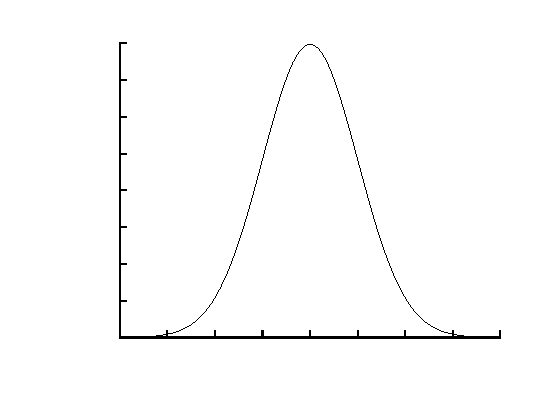
\includegraphics{fig_gauss}}%
    \gplfronttext
  \end{picture}%
\endgroup

\end{center}
\caption{A normal curve with mean zero and variance one, that is $\mu=0$ and $\sigma^2=1$.\label{fig_gauss}}
\end{figure}

The Gau\ss{}ian distribution is given by
\begin{equation}
p(x)=\frac{1}{\sqrt{2\pi\sigma^2}}e^{-\frac{(x-\mu)^2}{2\sigma^2}}
\end{equation}
It has a classic \lq{}bell\rq{} shape seen in Fig.~\ref{fig_gauss}; it
looks a bit like a binomial distribution with $p=0.5$. The slightly
confusing thing is the $1/\sqrt{2\pi\sigma^2}$, that is there to normalize the curve:
\begin{equation}
\int_{-\infty}^\infty e^{-x^2/2\sigma^2}dx=\sqrt{2\pi\sigma^2}
\end{equation}
This is confusing because we can do this particular definite integral
going from minus infinity to infinity, but the corresponding
indefinite integral can't be done in the sense that we can't write
down a formula in terms of functions we already know. There is a trick
for doing the definite integral from minus infinity to infinity which
we won't look at here for reasons of time but is very nice if you want
to look it up. Of course, since the integral goes from minus infinity
to infinity shifting the $x$ around doesn't change the value:
\begin{equation}
\int_{-\infty}^\infty e^{-(x-\mu)^2/2\sigma^2}dx=\sqrt{2\pi\sigma^2}
\end{equation}
where $\mu$ is a constant.

Surprisingly it is easier to calculate the moment generating function
than it is to calculate the mean and variance directly; we will do
this soon; we will see that the mean is $\mu$ and the variance
$\sigma^2$, just as we'd hope, that's why these particular symbols
were used in the formula for the density.

The Gau\ss{}ian distribution is sometimes described as
$\mathcal{N}(\mu,\sigma^2)$; this notation is a little confusing, it is never
really specified what \lq{}described as\rq{} means, but roughly
speaking people write $X\sim \mathcal{N}(\mu,\sigma^2)$ as a shorthand for say
$X$ is normally distributed with mean $\mu$ and variance $\sigma^2$

\subsection*{The moment generating function}

As we noted above, obviously when the constants were named $\mu$ and
$\sigma^2$ in the definition of the probability density it was because
these contants correspond to the mean and variance. Here we're going
to check that by working out the moment generating function for the
Gau\ss{}ian. This might seem a needlessly complicated way to work out
the mean and the variance, but it is actually the easiest way to do
it.

Recall that the moment generating function 
\begin{equation}
m(t)=\langle e^{tX}\rangle
\end{equation}
can be used to work out all the moments of a distribution. In the case of the Gau\ss{}ian
\begin{equation}
m(t)=\frac{1}{\sqrt{2\pi\sigma^2}}\int_{-\infty}^\infty e^{xt}e^{-\frac{(x-\mu)^2}{2\sigma^2}}dx
\end{equation}
Now $e^ae^b=e^{a+b}$ so
\begin{equation}
m(t)=\frac{1}{\sqrt{2\pi\sigma^2}}\int_{-\infty}^\infty e^{-\frac{(x-\mu)^2}{2\sigma^2}+xt}dx
\end{equation}
and we can complete the square: first add in the new term
\begin{equation}
\frac{(x-\mu)^2}{2\sigma^2}-xt=\frac{1}{2\sigma^2}(x^2-2\mu x +\mu^2-2\sigma^2 xt)
\end{equation}
Next add and take away what is needed to make a square
\begin{eqnarray}
x^2-2\mu x +\mu^2-2\sigma^2 xt &=& x^2-2(\mu+\sigma^2 t) x +(\mu+\sigma^2 t)^2 - 2\mu\sigma^2 t -\sigma^4 t^2\cr
                                &&= (x-\mu-\sigma^2 t)^2 - 2\mu\sigma^2 t -\sigma^4 t^2\
\end{eqnarray}
Hence
\begin{equation}
m(t)=\frac{1}{\sqrt{2\pi\sigma^2}}\int_{-\infty}^\infty e^{-\frac{(x-\mu-\sigma^2 t)^2}{2\sigma^2}+\mu t + \frac{1}{2}\sigma^2 t^2}dx
\end{equation}     
Finally use $e^{a+b}=e^ae^b$ and move stuff with no $x$s outside the integral
 \begin{equation}
m(t)=\left(\frac{1}{\sqrt{2\pi\sigma^2}}\int_{-\infty}^\infty e^{-\frac{(x-\mu-\sigma^2 t)^2}{2\sigma^2}}dx\right) e^{\mu t + \frac{1}{2}\sigma^2 t^2}
\end{equation}
and the stuff in the big brackets is just one, it is the integral of the Gau\ss{}ian with mean $\mu+\sigma^2 t$, so
\begin{equation}
m(t)= e^{\mu t + \frac{1}{2}\sigma^2 t^2}
\end{equation}

Now remember that 
\begin{equation}
\frac{d^nm}{dt^n}(0)=\mu_n
\end{equation}
where 
\begin{equation}
\mu_n=\langle X^n\rangle
\end{equation}
Now, using the chain rule, which in this case tells us that
\begin{equation}
\frac{d}{dt}e^{f(t)}=\frac{df}{dt}e^{f(t)}
\end{equation}
we get
\begin{equation}
\frac{d}{dt}e^{\mu t + \frac{1}{2}\sigma^2 t^2}=(\mu+\sigma^2 t)e^{\mu t + \frac{1}{2}\sigma^2 t^2}
\end{equation}
If we set $t=0$ this tells us that $\langle X\rangle =\mu$. Next
 \begin{equation}
\frac{d^2}{dt^2}e^{\mu t + \frac{1}{2}\sigma^2 t^2}=\frac{d}{dt}(\mu+\sigma^2 t)e^{\mu t + \frac{1}{2}\sigma^2 t^2}=[(\mu+\sigma^2 t)^2+\sigma^2]e^{\mu t + \frac{1}{2}\sigma^2 t^2}
\end{equation}
and if we set $t=0$ we get $\langle X^2\rangle =\sigma^2+\mu^2$ and
hence $\langle X^2\rangle-\langle X\rangle^2=\sigma^2$.

\subsection*{Working out Gau\ss{}ian probabilities}


\begin{figure}[tb]
\begin{center}
% GNUPLOT: LaTeX picture with Postscript
\begingroup
  \makeatletter
  \providecommand\color[2][]{%
    \GenericError{(gnuplot) \space\space\space\@spaces}{%
      Package color not loaded in conjunction with
      terminal option `colourtext'%
    }{See the gnuplot documentation for explanation.%
    }{Either use 'blacktext' in gnuplot or load the package
      color.sty in LaTeX.}%
    \renewcommand\color[2][]{}%
  }%
  \providecommand\includegraphics[2][]{%
    \GenericError{(gnuplot) \space\space\space\@spaces}{%
      Package graphicx or graphics not loaded%
    }{See the gnuplot documentation for explanation.%
    }{The gnuplot epslatex terminal needs graphicx.sty or graphics.sty.}%
    \renewcommand\includegraphics[2][]{}%
  }%
  \providecommand\rotatebox[2]{#2}%
  \@ifundefined{ifGPcolor}{%
    \newif\ifGPcolor
    \GPcolorfalse
  }{}%
  \@ifundefined{ifGPblacktext}{%
    \newif\ifGPblacktext
    \GPblacktexttrue
  }{}%
  % define a \g@addto@macro without @ in the name:
  \let\gplgaddtomacro\g@addto@macro
  % define empty templates for all commands taking text:
  \gdef\gplbacktext{}%
  \gdef\gplfronttext{}%
  \makeatother
  \ifGPblacktext
    % no textcolor at all
    \def\colorrgb#1{}%
    \def\colorgray#1{}%
  \else
    % gray or color?
    \ifGPcolor
      \def\colorrgb#1{\color[rgb]{#1}}%
      \def\colorgray#1{\color[gray]{#1}}%
      \expandafter\def\csname LTw\endcsname{\color{white}}%
      \expandafter\def\csname LTb\endcsname{\color{black}}%
      \expandafter\def\csname LTa\endcsname{\color{black}}%
      \expandafter\def\csname LT0\endcsname{\color[rgb]{1,0,0}}%
      \expandafter\def\csname LT1\endcsname{\color[rgb]{0,1,0}}%
      \expandafter\def\csname LT2\endcsname{\color[rgb]{0,0,1}}%
      \expandafter\def\csname LT3\endcsname{\color[rgb]{1,0,1}}%
      \expandafter\def\csname LT4\endcsname{\color[rgb]{0,1,1}}%
      \expandafter\def\csname LT5\endcsname{\color[rgb]{1,1,0}}%
      \expandafter\def\csname LT6\endcsname{\color[rgb]{0,0,0}}%
      \expandafter\def\csname LT7\endcsname{\color[rgb]{1,0.3,0}}%
      \expandafter\def\csname LT8\endcsname{\color[rgb]{0.5,0.5,0.5}}%
    \else
      % gray
      \def\colorrgb#1{\color{black}}%
      \def\colorgray#1{\color[gray]{#1}}%
      \expandafter\def\csname LTw\endcsname{\color{white}}%
      \expandafter\def\csname LTb\endcsname{\color{black}}%
      \expandafter\def\csname LTa\endcsname{\color{black}}%
      \expandafter\def\csname LT0\endcsname{\color{black}}%
      \expandafter\def\csname LT1\endcsname{\color{black}}%
      \expandafter\def\csname LT2\endcsname{\color{black}}%
      \expandafter\def\csname LT3\endcsname{\color{black}}%
      \expandafter\def\csname LT4\endcsname{\color{black}}%
      \expandafter\def\csname LT5\endcsname{\color{black}}%
      \expandafter\def\csname LT6\endcsname{\color{black}}%
      \expandafter\def\csname LT7\endcsname{\color{black}}%
      \expandafter\def\csname LT8\endcsname{\color{black}}%
    \fi
  \fi
  \setlength{\unitlength}{0.0500bp}%
  \begin{picture}(5040.00,3528.00)%
    \gplgaddtomacro\gplbacktext{%
      \csname LTb\endcsname%
      \put(462,439){\makebox(0,0)[r]{\strut{} 0}}%
      \put(2619,220){\makebox(0,0){\strut{} $\mu$}}%
      \put(2872,220){\makebox(0,0){\strut{} $z_1$}}%
      \put(3479,220){\makebox(0,0){\strut{} $z_2$}}%
    }%
    \gplgaddtomacro\gplfronttext{%
    }%
    \gplbacktext
    \put(0,0){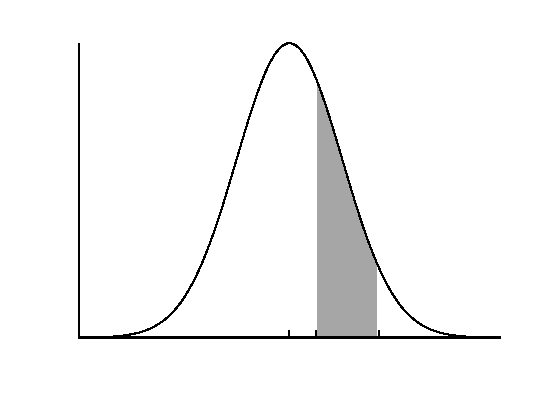
\includegraphics{fig_prob}}%
    \gplfronttext
  \end{picture}%
\endgroup

\end{center}
\caption{Working out the probability means calculating the area under the curve.\label{fig_prob}}
\end{figure}


\begin{figure}[tb]
\begin{center}
% GNUPLOT: LaTeX picture with Postscript
\begingroup
  \makeatletter
  \providecommand\color[2][]{%
    \GenericError{(gnuplot) \space\space\space\@spaces}{%
      Package color not loaded in conjunction with
      terminal option `colourtext'%
    }{See the gnuplot documentation for explanation.%
    }{Either use 'blacktext' in gnuplot or load the package
      color.sty in LaTeX.}%
    \renewcommand\color[2][]{}%
  }%
  \providecommand\includegraphics[2][]{%
    \GenericError{(gnuplot) \space\space\space\@spaces}{%
      Package graphicx or graphics not loaded%
    }{See the gnuplot documentation for explanation.%
    }{The gnuplot epslatex terminal needs graphicx.sty or graphics.sty.}%
    \renewcommand\includegraphics[2][]{}%
  }%
  \providecommand\rotatebox[2]{#2}%
  \@ifundefined{ifGPcolor}{%
    \newif\ifGPcolor
    \GPcolorfalse
  }{}%
  \@ifundefined{ifGPblacktext}{%
    \newif\ifGPblacktext
    \GPblacktexttrue
  }{}%
  % define a \g@addto@macro without @ in the name:
  \let\gplgaddtomacro\g@addto@macro
  % define empty templates for all commands taking text:
  \gdef\gplbacktext{}%
  \gdef\gplfronttext{}%
  \makeatother
  \ifGPblacktext
    % no textcolor at all
    \def\colorrgb#1{}%
    \def\colorgray#1{}%
  \else
    % gray or color?
    \ifGPcolor
      \def\colorrgb#1{\color[rgb]{#1}}%
      \def\colorgray#1{\color[gray]{#1}}%
      \expandafter\def\csname LTw\endcsname{\color{white}}%
      \expandafter\def\csname LTb\endcsname{\color{black}}%
      \expandafter\def\csname LTa\endcsname{\color{black}}%
      \expandafter\def\csname LT0\endcsname{\color[rgb]{1,0,0}}%
      \expandafter\def\csname LT1\endcsname{\color[rgb]{0,1,0}}%
      \expandafter\def\csname LT2\endcsname{\color[rgb]{0,0,1}}%
      \expandafter\def\csname LT3\endcsname{\color[rgb]{1,0,1}}%
      \expandafter\def\csname LT4\endcsname{\color[rgb]{0,1,1}}%
      \expandafter\def\csname LT5\endcsname{\color[rgb]{1,1,0}}%
      \expandafter\def\csname LT6\endcsname{\color[rgb]{0,0,0}}%
      \expandafter\def\csname LT7\endcsname{\color[rgb]{1,0.3,0}}%
      \expandafter\def\csname LT8\endcsname{\color[rgb]{0.5,0.5,0.5}}%
    \else
      % gray
      \def\colorrgb#1{\color{black}}%
      \def\colorgray#1{\color[gray]{#1}}%
      \expandafter\def\csname LTw\endcsname{\color{white}}%
      \expandafter\def\csname LTb\endcsname{\color{black}}%
      \expandafter\def\csname LTa\endcsname{\color{black}}%
      \expandafter\def\csname LT0\endcsname{\color{black}}%
      \expandafter\def\csname LT1\endcsname{\color{black}}%
      \expandafter\def\csname LT2\endcsname{\color{black}}%
      \expandafter\def\csname LT3\endcsname{\color{black}}%
      \expandafter\def\csname LT4\endcsname{\color{black}}%
      \expandafter\def\csname LT5\endcsname{\color{black}}%
      \expandafter\def\csname LT6\endcsname{\color{black}}%
      \expandafter\def\csname LT7\endcsname{\color{black}}%
      \expandafter\def\csname LT8\endcsname{\color{black}}%
    \fi
  \fi
  \setlength{\unitlength}{0.0500bp}%
  \begin{picture}(5040.00,3528.00)%
    \gplgaddtomacro\gplbacktext{%
      \csname LTb\endcsname%
      \put(726,440){\makebox(0,0)[r]{\strut{}-1}}%
      \put(726,1146){\makebox(0,0)[r]{\strut{}-0.5}}%
      \put(726,1852){\makebox(0,0)[r]{\strut{} 0}}%
      \put(726,2557){\makebox(0,0)[r]{\strut{} 0.5}}%
      \put(726,3263){\makebox(0,0)[r]{\strut{} 1}}%
      \put(858,220){\makebox(0,0){\strut{}-4}}%
      \put(1331,220){\makebox(0,0){\strut{}-3}}%
      \put(1804,220){\makebox(0,0){\strut{}-2}}%
      \put(2277,220){\makebox(0,0){\strut{}-1}}%
      \put(2751,220){\makebox(0,0){\strut{} 0}}%
      \put(3224,220){\makebox(0,0){\strut{} 1}}%
      \put(3697,220){\makebox(0,0){\strut{} 2}}%
      \put(4170,220){\makebox(0,0){\strut{} 3}}%
      \put(4643,220){\makebox(0,0){\strut{} 4}}%
    }%
    \gplgaddtomacro\gplfronttext{%
    }%
    \gplbacktext
    \put(0,0){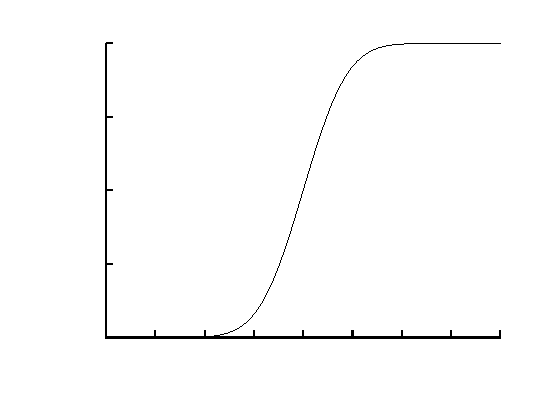
\includegraphics{fig_erf}}%
    \gplfronttext
  \end{picture}%
\endgroup

\end{center}
\caption{The error function $\mbox{erf}(x)$.\label{fig_erf}}
\end{figure}


Obviously what we'd like to do is work out probabilities:
\begin{equation}
\mbox{Prob}(x_1<x<x_2)=\frac{1}{\sqrt{2\pi\sigma^2}}\int_{x_1}^{x_2} e^{-\frac{(x-\mu)^2}{2\sigma^2}}dx
\end{equation}
as illustrated in Fig.~\ref{fig_prob}. The problem is that we can't
do that integral, there is no way to write the integral in terms of
function we already know. The solution to this problem is to define a
new function, \textsl{the error function}, specifically for using to
do the integral:
\begin{equation}
\mbox{erf}\,(x)=\frac{1}{\sqrt{\pi}}\int_{-x}^xe^{-y^2}dy=\frac{2}{\sqrt{\pi}}\int_0^xe^{-y^2}dy
\end{equation}
This is a so called \textsl{special function} which rougly means a
function we needed to define so that we could do an integral, or solve
a differential equation, we couldn't otherwise do or solve. Other
examples are Bessel functions and the elliptic integrals; there are
lots, especially coming from applied mathematics. Sometimes some
number theory functions, like Euler's totient function, are called
special functions. A lot of effort in the C19 was put into defining
special functions and finding efficient ways to numerically calculate
values; in those days, of course, these then went into big tables of
values; now all of that is done for us by the C \texttt{math} library
and it successors.

A graph of $\mbox{erf}\,(x)$ is shown in Fig.~\ref{fig_erf}. We can use it to work out Gau\ss{}ian probablities. Consider
\begin{equation}
\mbox{Prob}(x_1<x<x_2)=\int_{x_!}^{x_2} p(x)dx=\frac{1}{\sqrt{2\pi\sigma^2}}\int_{x_1}^{x_2} e^{-\frac{(x-\mu)^2}{2\sigma^2}}dx 
\end{equation}
Now let
\begin{equation}
z=\frac{x-\mu}{\sqrt{2}\sigma}
\end{equation}
so 
\begin{equation}
dz=\frac{dx}{\sqrt{2}\sigma}
\end{equation}
and when $x=x_1$ we have
\begin{equation}
z=z_1=\frac{x_1-\mu}{\sqrt{2}\sigma}
\end{equation}
and when $x=x_2$ we have
\begin{equation}
z=z_2=\frac{x_2-\mu}{\sqrt{2}\sigma}
\end{equation}
Substituting this all back into the integral
\begin{equation}
\mbox{Prob}(x_1<y<x_2)=\frac{1}{\sqrt{\pi}}\int_{z_1}^{z_2} e^{-\frac{z^2}{2}}dz=\frac{1}{\sqrt{\pi}}\int_{z_1}^{0} e^{-z^2}dz+\frac{1}{\sqrt{\pi}}\int_{0}^{z_2} e^{-z^2}dz
\end{equation}
Hence using the usual 
\begin{equation}
\int_a^bf(x)dx=-\int_b^a f(x)dx
\end{equation}
we have
\begin{equation}
\mbox{Prob}(x_1<x<x_2)=\frac{1}{2}[\mbox{erf}\,(z_2)-\mbox{erf}\,(z_1)]
\end{equation}

\subsection*{Example}

The loudness of songs at a concert are normally distributed with mean 75 dB and standard deviation $\sigma=10 dB$. What is the probability that the next song has loudness between 80 and 90 dB? Well
\begin{equation}
\mbox{Prob}(80<x<90)=\frac{1}{2}[\mbox{erf}\,(z_2)-\mbox{erf}\,(z_1)]
\end{equation}
where 
\begin{equation}
\sqrt{2}z_1=\frac{80-75}{10}=0.5
\end{equation}
and 
\begin{equation}
\sqrt{2}z_2=\frac{90-75}{10}=1.5
\end{equation}
Working out $\mbox{erf}\,(0.5/\sqrt{2})$ using your calculator or computer gives 0.38, whereas $\mbox{erf}\,(1.5/\sqrt{2})=0.87$ so
\begin{equation}
\mbox{Prob}(80<x<90)=0.2417
\end{equation}

\end{document}




